The goal of this chapter is to offer the theoretical basis for ideas that are assumed but not elaborated in \refCap{3-TrabalhosRelacionados} and \refCap{4-Metodologia}.

\section{Traditional Classification}

It is mentioned very often in this paper that traditional classification cannot generalize over unseen classes. In the context of this work, it can be specified further: \gls{DL} models, trained with a cross-entropy learning framework, cannot classify an element into a class that has not been mapped beforehand. This is because the model is trained to minimize the cross-entropy loss function over a labeled dataset, associating each input with a fixed class label. For a single instance, the cross-entropy equation is as follows:

\begin{equation}
    \label{cross_entropy}
    \begin{split}
        CE_{loss} = & -\sum_{c=1}^My_{c}\log(p_{c}),
    \end{split}
\end{equation}

where $p_{c}$ denotes the predicted probability of the input element belonging to class $c$, $y_{c}$ is a label that is $1$ if the element belongs to $c$, and $0$ otherwise, and $M$ is the number of classes. When a model is trained using a class-disjoint split, meaning that no class appears in both training and test sets, a cross-entropy classifier is unable to learn anything about the unseen classes. Since these classes are not represented in the training data, it is not possible to compute a meaningful cross-entropy loss for them. Therefore, to tackle \gls{ZSL}, another approach is needed.

\section{Metric Learning}

Metric learning is a framework that allows \gls{ZSL}. In summary, a metric-learning model \( f(\cdot) \) is trained such that, over an input element, it yields a feature vector $v$, instead of a traditional classification. This model \( f(\cdot) \) is optimized under a given metric \( d(\cdot, \cdot) \), such that two feature vectors that share the same class $v_1$, $v_1'$ are closer together than two feature vectors from different classes $v_1$, $v_2$. In other words, the model is optimized so that $d(v_1, v_1') < d(v_1, v_2)$ and $d(v_1, v_1') < d(v_1', v_2)$.

A \gls{DL} model following a metric learning framework is constructed as a siamese network. They are named siamese because they can be seen as bipartite architectures, with two parallel paths that converge in the end, even though both sides share the same weights. To construct a visual siamese network, an image model, \( g(\cdot) \), is required to transform an input image \( I \) into a feature representation in an arbitrary $n$-dimensional space, \( g(I) \). The  \( g(\cdot) \) image model is referred to as the backbone of the siamese network. This framework is illustrated in Figure \ref{fig:siamese} for reference.

\begin{figure}[htbp]
%\isPreprints{\centering}{} % Only used for preprints
\centering
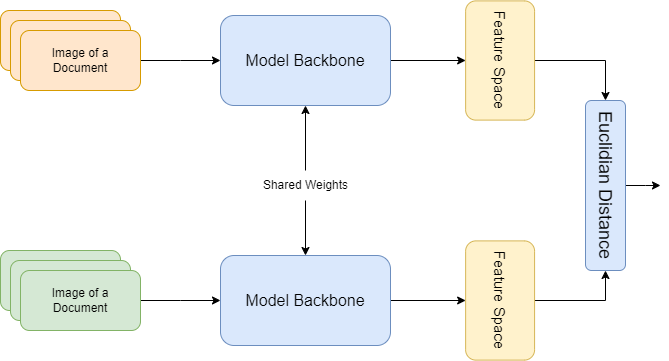
\includegraphics[width=0.9\linewidth]{images/siamese.png}
\caption{Simplified architecture of a siamese network}
\label{fig:siamese}
\end{figure}

The metric learning nature of this method makes it highly adaptable to different applications. Since feature vectors are used, clustering is a very natural application of the method, as are verification and identification. By establishing a distance threshold, it is possible to declare that two elements are similar enough to be considered a positive case, or far enough to be a negative case. Using this strategy, and having a reference for each required class, verification can be performed by comparing a given element with a certain class, effectively employing binary classification, or identification can be performed by comparing the element with every class and taking the most similar, effectively employing multiclass classification.

Losses that support metric learning, such as contrastive~\cite{chopra_learning_2005} or triplet~\cite{hoffer_deep_2018}, follow the same strategy: cluster together elements that share a label, and split apart elements that do not. When training a siamese network, the training step should consider at least two distinct elements, and the loss function scores the step over the distance between the elements. During training, the contrastive loss considers only two elements per step, and they can either share the same class or belong to different classes. The triplet loss considers three elements per step: an anchor/reference, a positive example (same label), and a negative example (different label). In this work, the contrastive loss function is used to train the model.

\subsection{Contrastive Loss}

The contrastive loss function  $\mathcal{L}$=$\mathcal{L}(m, y, x_1, x_2)$ is defined as follows:
\begin{equation}
    \mathcal{L} = y \cdot d(x_1, x_2)^2 + (1 - y) \cdot abs(m - d(x_1, x_2))^2,
\end{equation}
where $d$ metric function, $m > 0$ is a hyperparameter defining a distance margin representing the boundary to discriminate what is different and what is similar, such as $(x_1, x_2)$ are a positive input pair of documents. Lastly, $y$ is a label with value $1$, if both elements share the same class, or $0$ otherwise. Therefore, the loss function can be alternatively expressed as
\begin{equation}
    \mathcal{L} = \begin{cases}
        d(x_1, x_2)^2, & \text{if } y = 1 \\
        abs(m - d(x_1, x_2))^2, & \text{otherwise}.
  \end{cases}
\end{equation}
\vspace{1em}

In this context of this paper, $d$ is the Euclidean distance between two points $P = (x_{11}, x_{12}, \cdots, x_{1n})$ and $Q = (x_{21}, x_{22}, \cdots, x_{2n})$ in an $n$-dimensional space defined mathematically as:
\begin{equation}
d(P,Q)={\sqrt {(x_{11}-x_{21})^{2}+ \cdots +(x_{1n}-x_{2n})^{2}}} = \sqrt{ \sum_{i=1}^{n} (x_1i - x_2i)^2 }.
\end{equation}

% Therefore, given a sample pair $\{(a, b)\}$ of feature spaces, and $y$ as a label with value $1$ if $a$ and $b$ share the same class, $0$ otherwise, the contrastive loss can be defined as:
% \begin{equation}
%         Loss = y * d(a, b)^2 + (1 + (-1 * y)) * abs(m - d(a, b))^2,
% \end{equation}
% where $d$ represents a metric function and $m$ a hyperparameter defining the lower bound distance between samples of different classes. In this context of this paper, $d$ is the Euclidean distance between two points $P = (x_1, x_2, \cdots, x_n)$ and $Q = (y_1, y_2, \cdots, y_n)$ in an $n$-dimensional space defined mathematically as:
% \begin{equation}
% d(P,Q)={\sqrt {(x_{1}-y_{1})^{2}+ \cdots +(x_{n}-y_{n})^{2}}} = \sqrt{ \sum_{i=1}^{n} (x_i - y_i)^2 }.
% \end{equation}


% \section{Vision Models}

% \gls{DL} vision models are defined by their capability to analyze and generate predictions over images~\cite{trigka_comprehensive_2025}. In general, these models receive images codified as pixel matrixes $(C,H,W)$, where $C$ is the number of color channels in the image and $H$ and $W$ are the height and width of the image in number of pixels. Vision models can tackle a wide variety of tasks, such as image classification~\cite{deng_imagenet_2009}, image segmentation~\cite{ronneberger_u-net_2015} and object detection~\cite{redmon_you_2016}. Most 

\section{Large Language Models}

\glspl{LLM} are \gls{DL} networks trained on massive corpora of textual data to, traditionally, generate human-like text, although they can be adapted to a number of different tasks. Modern LLMs, such as GPT~\cite{brown_language_2020} and LLaMA~\cite{touvron_llama_2023}, have demonstrated remarkable performance across a wide variety of \gls{NLP} tasks. One of the defining characteristics of LLMs is their ability to generalize to unseen tasks without task-specific fine-tuning, a phenomenon often referred to as in-context learning. Instead of retraining the model, a user can provide a prompt containing instructions or examples, and the model adapts its behavior accordingly. This makes LLMs particularly appealing for applications where labeled data is scarce or non-existent, excelling in zero-shot and few-shot tasks.

Despite their versatility, LLMs come with challenges. Their performance can degrade in highly specialized domains or when exposed to out-of-distribution inputs. Generative LLMs in particular are very susceptible to hallucination~\cite{ji_survey_2023}, where the output answer is structurally correct but has no connection to the input text, or even has fabricated information. In a corporate scenario, integrating a generative LLM into an automation pipeline is particularly challenging. Many systems depend on structured communication, and a generative model may hallucinate on the structure itself, breaking the system even if the answer was semantically correct. Even then, they continue to shape current research and development in machine learning, and their integration into hybrid or multimodal systems is a growing area of interest.

\subsection{Vision Language Models}

\glspl{VLM} are multimodal versions of the \glspl{LLM}. They both follow the same constraints, except the \gls{VLM} receives and understands both image and text inputs, enabling the model to perform tasks such as image captioning, visual question answering, \gls{OCR}, and document understanding. While \glspl{LLM} show great zero-shot performance across various \gls{NLP} tasks, \glspl{VLM} can perform in vision-related problems as well, making them particularly useful in the document analysis scenario.

\section{Active Learning}
\label{sec:active_learning}

Active learning~\cite{settles_active_2009} is a machine learning paradigm that focuses on optimizing the labeling process. It is especially helpful in scenarios where resources are scarce or the target dataset is aimed to be particularly large. This process reduces the labeling cost by using the trained model itself to help gather more labeled data. This process can be visualized in \refFig{fig:activelearning}.

To use this approach, first, a small labeled dataset must be generated to start the process. This first step can be the most laborious, as there is not an auxiliary trained model yet. Then, a machine learning model must be trained with this data. This model is then used to evaluate a larger pool of unlabeled data and predict their labels. Then, the predicted labels are returned to a human hand to validate and correct the produced labels. There are many strategies to further optimize this process, such as identifying instances where the model's predictions are uncertain or where the data points are expected to provide the most information gain if labeled. This process can be repeated as many times as needed, achieving a better model and a larger dataset at each iteration.

\begin{figure}[htbp]
%\isPreprints{\centering}{} % Only used for preprints
\centering
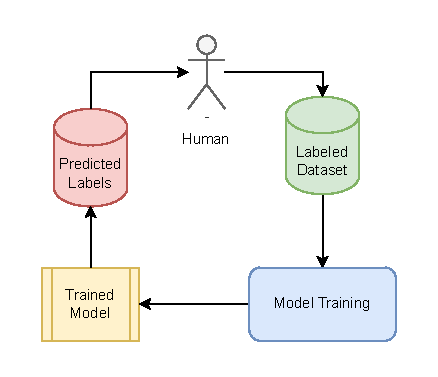
\includegraphics[width=.6\linewidth]{images/active_learning.drawio.pdf}
\caption{Simplified diagram of an active learning process.}
\label{fig:activelearning}
\end{figure}